\begin{frame}[fragile,label=infoFlowExample1a]{information flow graph (1a)}
\begin{lstlisting}[language=Python,style=smaller]
def f(a, b, c):
    desc = 'a={},b={}'.format(a, b)
    if b > 10:
        y = a
    else:
        y = c
    w = y + a
    pair = (w, c)
    desc = desc + \
         ',pair={}'.format(pair)
    print(desc)
    return y
\end{lstlisting}
\begin{tikzpicture}[overlay,remember picture]
\node[anchor=north east] at ([xshift=-.25cm,yshift=-1cm]current page.north east) {
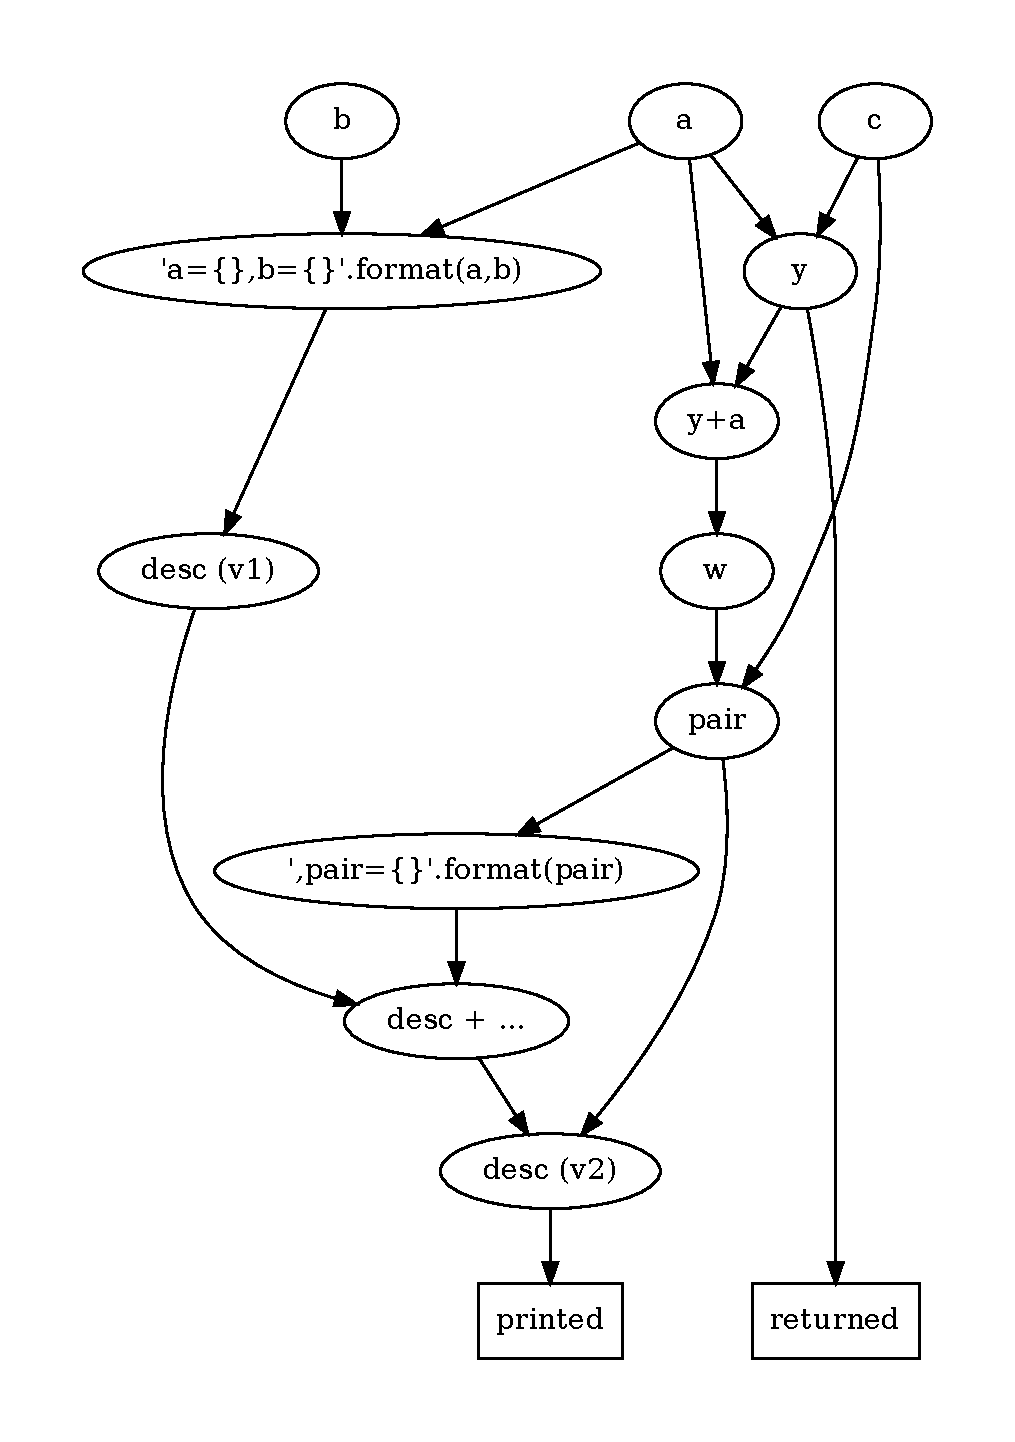
\includegraphics[width=0.4\textwidth]{../taint/info-flow-graph1}
};
\end{tikzpicture}
\end{frame}

\begin{frame}[fragile,label=infoFlowExample1b]{information flow graph (1b)}
\begin{itemize}
\item<2-> ex: does returned value depend on a, b, c?
\item<2-> ex: does value of pair depend on a, b, c?
\item<2-> ex: does printed value depend on a, b, c?
\end{itemize}
\begin{tikzpicture}[overlay,remember picture]
\node[anchor=north east] at ([xshift=-.25cm,yshift=-1cm]current page.north east) {
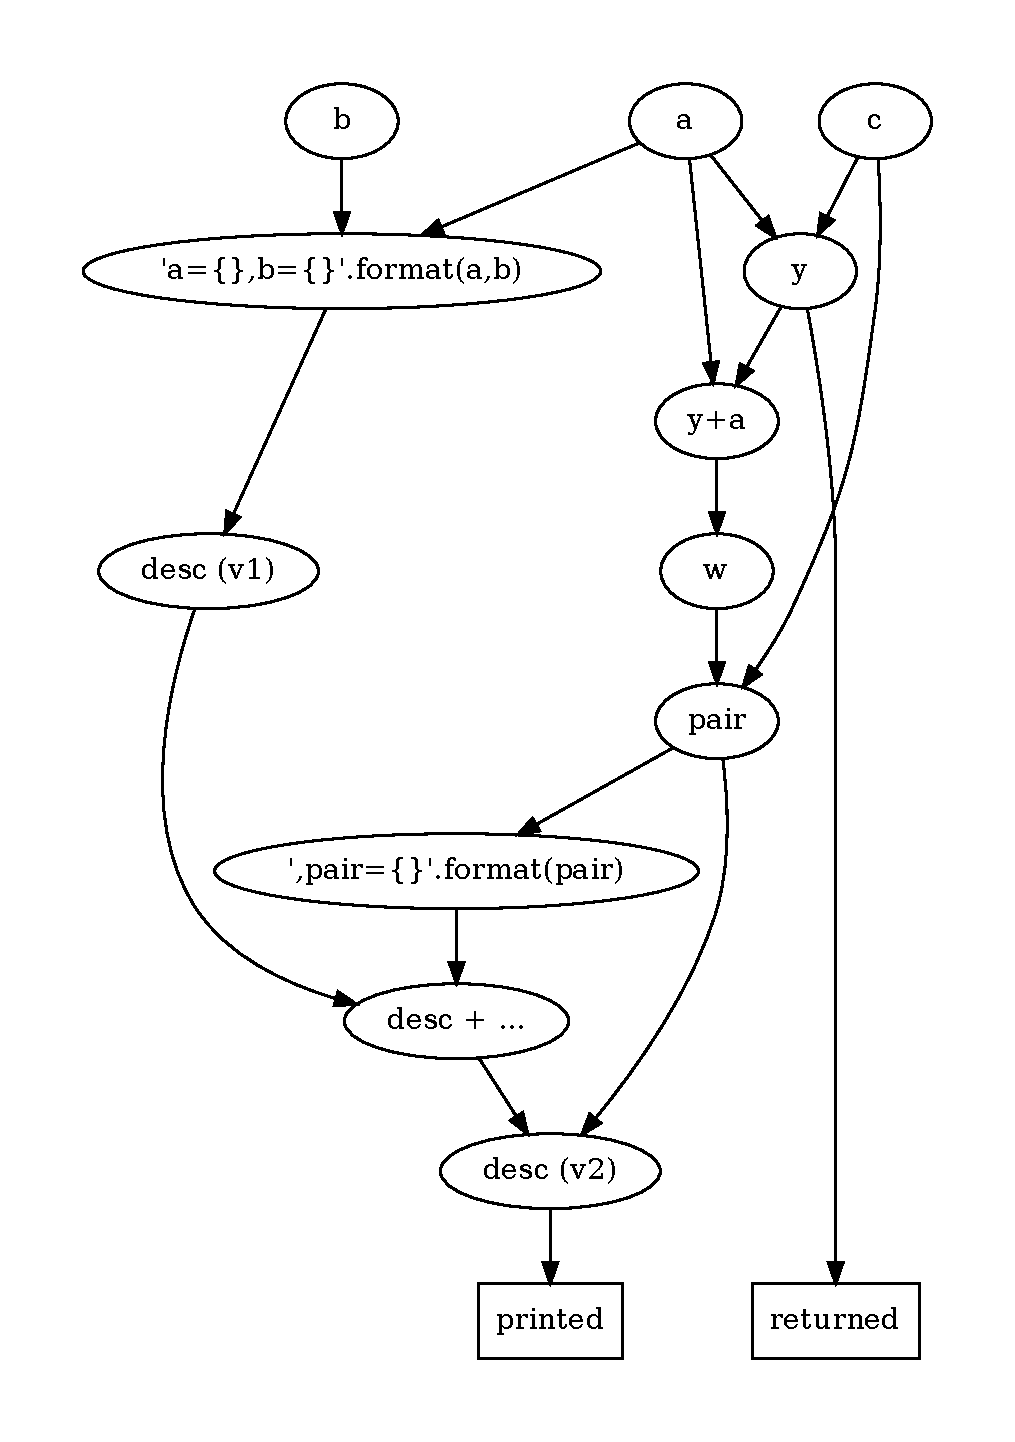
\includegraphics[width=0.4\textwidth]{../taint/info-flow-graph1}
};
\end{tikzpicture}
\end{frame}
